\documentclass{tufte-handout}

%\geometry{showframe}% for debugging purposes -- displays the margins

\usepackage{amsmath}

% Set up the images/graphics package
\usepackage{graphicx}
\setkeys{Gin}{width=\linewidth,totalheight=\textheight,keepaspectratio}
\graphicspath{{graphics/}}

\title{Intro to Research Data Management for PoliSci}
\author[Michelle Hudson]{Michelle Hudson}
\date{Fall 2014}  % if the \date{} command is left out, the current date will be used

% The following package makes prettier tables.  We're all about the bling!
\usepackage{booktabs}

% The units package provides nice, non-stacked fractions and better spacing
% for units.
\usepackage{units}

% The fancyvrb package lets us customize the formatting of verbatim
% environments.  We use a slightly smaller font.
\usepackage{fancyvrb}
\fvset{fontsize=\normalsize}

% Small sections of multiple columns
\usepackage{multicol}

% Provides paragraphs of dummy text
\usepackage{lipsum}

% These commands are used to pretty-print LaTeX commands
\newcommand{\doccmd}[1]{\texttt{\textbackslash#1}}% command name -- adds backslash automatically
\newcommand{\docopt}[1]{\ensuremath{\langle}\textrm{\textit{#1}}\ensuremath{\rangle}}% optional command argument
\newcommand{\docarg}[1]{\textrm{\textit{#1}}}% (required) command argument
\newenvironment{docspec}{\begin{quote}\noindent}{\end{quote}}% command specification environment
\newcommand{\docenv}[1]{\textsf{#1}}% environment name
\newcommand{\docpkg}[1]{\texttt{#1}}% package name
\newcommand{\doccls}[1]{\texttt{#1}}% document class name
\newcommand{\docclsopt}[1]{\texttt{#1}}% document class option name

\begin{document}

\maketitle% this prints the handout title, author, and date
 
\paragraph{\href{https://github.com/michellehudson/datamanagement/}{https://github.com/michellehudson/datamanagement/}}\label{httpsgithub.commichellehudsondatamanagement} 

\marginnote {\href{mailto:michelle.hudson@yale.edu}{michelle.hudson@yale.edu} \href{mailto:melanie.maksin@yale.edu}{melanie.maksin@yale.edu}}

\marginnote {\subsection{Helpful guides:}\label{guides}
\href{http://guides.library.yale.edu/datamanagement}{http://guides.library.yale.edu/datamanagement}
\href{http://guides.library.yale.edu/data-statistics}{http://guides.library.yale.edu/data-statistics} 
\href{http://guides.library.yale.edu/eln}{http://guides.library.yale.edu/eln}
\href{http://csssi.yale.edu/datamanagement}{http://csssi.yale.edu/datamanagement}}

\marginnote {\subsection{More resources:}\label{additional-help}

\href{http://statlab.stat.yale.edu/workshops/}{CSSSI Workshops: http://statlab.stat.yale.edu/workshops/} 
\smallskip
\newline
\href{http://its.yale.edu/services/research-technologies/high-performance-computing}{High Performance Computing: http://its.yale.edu/services/research-technologies/high-performance-computing} 
\medskip
\newline
\href{http://guides.library.yale.edu/gis}{Geographic Information Systems: http://guides.library.yale.edu/gis}}


\section{Overview:}\label{overview}
Using the DDI data lifecycle model as a guide, this workshop will cover the following
questions: 

\begin{enumerate}
\def\labelenumi{\arabic{enumi}.}
\itemsep1pt\parskip0pt\parsep0pt
\item
  What does this stage of the data lifecycle involve?
\item
  What resources are available for doing it well at Yale (\& elsewhere)?
\item
  What are guidelines for managing data at this stage?
\end{enumerate}


\begin{figure}
  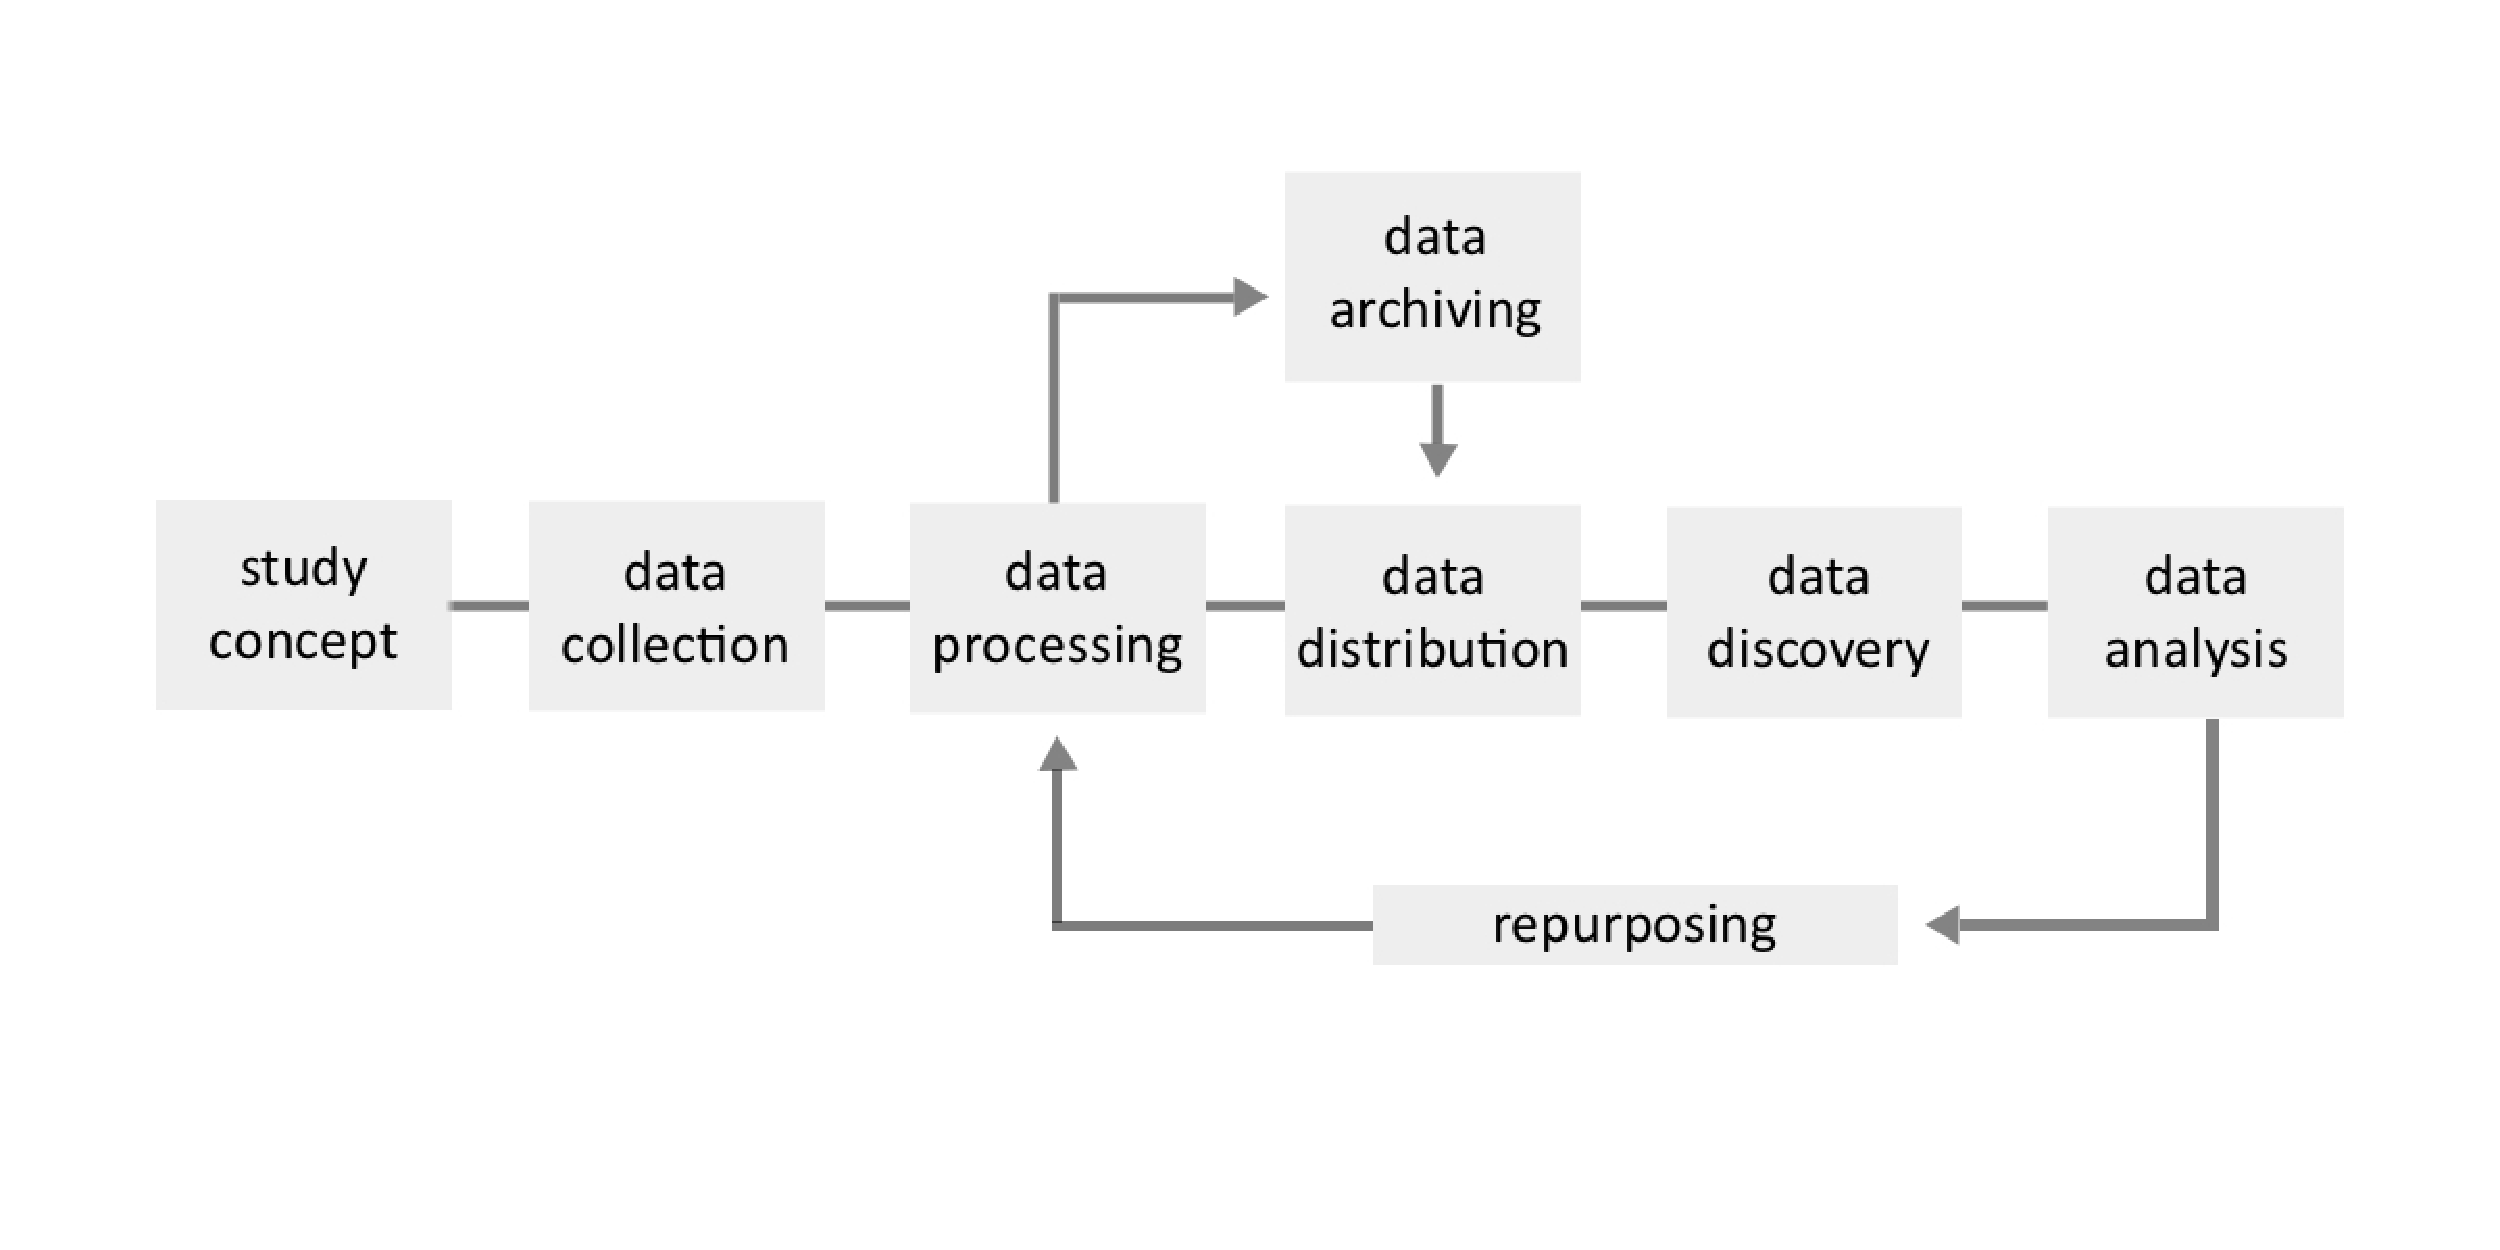
\includegraphics{ddilifecycle.pdf}
%  \checkparity This is an \pageparity\ page.%
  \caption{Data lifecycle model based on DDI.}
  \label{fig:textfig}
  %\zsavepos{pos:textfig}
  \setfloatalignment{b}
\end{figure}

\section{What is research data?}\label{what-is-research-data}

Research data is defined as ``the recorded factual material commonly
accepted in the scientific community as necessary to validate research
findings.'' \footnote {OMB Circular A-110.} 

\marginnote {

\bigskip

Research data comes in many formats of information: documents,
spreadsheets, field notebooks, survey responses, audio and video
recordings, images, film, specimens, software code, and can be
structured and stored in a variety of file formats.}

\begin{enumerate}
\def\labelenumi{\arabic{enumi}.}
\itemsep1pt\parskip0pt\parsep0pt
\item
  Observational: captured in real time, usually irreplaceable (sensor readings, telescope images, sample data, surveys).
\item
  Experimental: data from lab equipment, can be reproducible but may be expensive (gene sequences).
\item
  Simulation: data generated from test models (climate models).
\item
  Derived or compiled: reproducible but expensive (data mining, compiled databases).
\end{enumerate}

\newpage

\marginnote {\subsection{Guidelines:}\label{guidelines-concept}
\begin{enumerate}
\def\labelenumi{\arabic{enumi}.}
\itemsep1pt\parskip0pt\parsep0pt
\item
  Visit the CSSSI before you start your project.
\item
  Consider making a data management plan even if you aren't seeking a grant.

\end{enumerate}}
\vspace*{-50pt}
\section{Study concept}\label{study-concept}

\paragraph{\href{https://dmptool.org}{DMPTool https://dmptool.org}}\label{dmptool}

\paragraph{\href{http://csssi.yale.edu/dmp}{Data Management Consultation
Group http://csssi.yale.edu/dmp}}\label{dmp-consultation-group}

\paragraph{\href{http://csssi.yale.edu/csssi-statistical-consultants-schedule}{Datta
consultants http://csssi.yale.edu/csssi-statistical-consultants-schedule} }\label{data-consultants}

\marginnote
{\subsection{Guidelines for data collection \& documentation:}\label{guidelines-doc}
\begin{enumerate}
\def\labelenumi{\arabic{enumi}.}
\itemsep1pt\parskip0pt\parsep0pt
\item
  Look at great examples of documentation, like the General Social Survey.
\item
  Consistency: whatever you do, stick with it.
\item
  Level of detail: What would someone need to know to re-use your data or replicate your findings?
\end{enumerate}}

\section{Data collection \& documentation}\label{data-collection-documentation}

\subsection{Yale-supported resources:}\label{yale-supported}

\begin{itemize}
\item
  \href{http://its.yale.edu/services/collaboration-and-file-sharing/box-yale}{Box}
\item
  \href{http://its.yale.edu/services/research-technologies/elab-notebook/labarchives-faqs}{LabArchives}
\item
  \href{http://its.yale.edu/services/email-and-calendars/eliapps-google-apps-education}{EliApps}
\item
  \href{http://its.yale.edu/services/web-and-application-services/qualtrics-survey-tool}{Qualtrics}
\item
  \href{http://its.yale.edu/services/web-and-application-services/github-enterprise}{GitHub}
\end{itemize}

\marginnote{\subsection{Guidelines for data processing \& analysis:}\label{guidelines-processing}
\begin{enumerate}
\def\labelenumi{\arabic{enumi}.}
\itemsep1pt\parskip0pt\parsep0pt
\item
  Visit the CSSSI before you start your project.
\item
  Keep track of everything you do and always keep versions of your data
  sets.
\item
  Best practices for working with data during analysis -- folder
  structures, naming conventions, statistical package considerations.
\item
  Back up data in accordance with good practice.
\end{enumerate}}


\section{Data processing \& analysis}\label{data-processing-analysis}

\begin{itemize}
\itemsep1pt\parskip0pt\parsep0pt
\item
  Stata, SAS, MatLab, R, OpenRefine, Python
\item
  \href{http://www.dataone.org/software_tools_catalog}{DataONE software tools catalog}
  \item
  \href{http://csssi.yale.edu/tech}{Tech at CSSSI}
\end{itemize}



\marginnote{\subsection{Guidelines for data archiving \& preservation:}\label{guidelines-preservation}

\begin{enumerate}
\def\labelenumi{\arabic{enumi}.}
\itemsep1pt\parskip0pt\parsep0pt
\item 
  Backup is not sufficient for preservation.
\item
  Doing preservation yourself requires format migration and ensuring integrity of files.
\item
  Handing over your data to a repository like ICPSR is possible, and will ensure the data is usable over the long-term.
\end{enumerate}}


\section{Data archiving, preservation, distribution, and citation:}\label{data-archiving-preservation} 

\begin{itemize}
\itemsep1pt\parskip0pt\parsep0pt
\item
  \href{https://www.datacite.org/}{DataCite https://www.datacite.org/}
\item
 \href{http://www.re3data.org}{re3data http://www.re3data.org}
\item
\href{http://databib.org/}{DataBib http://databib.org/}
\end{itemize}

\marginnote {\subsection{Guidelines for data distribution \& citation:}\label{guidelines-citation}

\begin{enumerate}
\def\labelenumi{\arabic{enumi}.}
\itemsep1pt\parskip0pt\parsep0pt
\item
  Give your data set a title and make it easy to credit you.
\item
  Always cite data that you use as if it were as important as the  journal articles you cite.
\item
  Look for domain-appropriate distribution channels.
\end{enumerate}}

\subsection{Additional services \& software:}\label{additional-services-software}

\begin{itemize}
\item
  \href{https://github.com/}{GitHub}: https://github.com/
\item
  \href{https://knb.ecoinformatics.org/morphoportal.jsp}{Morpho}
  https://knb.ecoinformatics.org/morphoportal.jsp 
\item
  \href{http://earthcube.org/}{Earthcube} http://earthcube.org/
\item
  \href{http://www.colectica.com/}{Colectica} http://www.colectica.com/
\end{itemize}


\end{document}
